\documentclass[a4paper ,11pt]{report}
\usepackage[top=2.5cm, bottom=2.5cm, left=2.5cm, right=2.5cm]{geometry}
\usepackage{ucs}
\usepackage{url}
\usepackage{graphicx}
\usepackage[utf8x]{inputenc} % ou utf8x au lieu
\usepackage[T1]{fontenc} % de latin 1
\usepackage{lmodern}
\usepackage[french]{babel}
\usepackage{listings}
\usepackage{subfigure}
\renewcommand{\familydefault}{\sfdefault}


\begin{document}
\begin{titlepage}
\begin{center}
\begin{figure}
    \includegraphics[height=3cm]{Eurobot.png}
   	\hfill
    \includegraphics[height=3cm]{ecam.jpg}
\end{figure}
\end{center}
\vspace{4cm}
\begin{center}
	{\Huge Eurobot 2014--2015, BetterWithMotors\\}
	{\huge Rapport intermédiaire\\}
	\vspace{1.5cm}
	José-Carlos Alves Da Costa\\
	Mounïme Bouzanih\\
	Louis Defauw\\
	Arnaud Iserentant\\
	Abdelhak Kotati\\
	Nabil Nehri\\
	Alexis Paques
	\vfill
	\today
\end{center}
\end{titlepage}

\tableofcontents

\chapter{Gestion}


%gestion
\section{Méthode SCRUM}
%~~~~~~~~~~~~~~~~~~~~~~~~~~~~~~~~~~~~~~~~~~~~~~~~~~~~~~~~~~~~
\subsection{Organisation}
\paragraph{}
Dans l'optique du projet robot, nous avons suivi une méthode agile, SCRUM, qui correspondait à nos besoins d'organisation. En effet, pour un travail en comité réduit avec une échéance suffisamment longue, cette méthode offre un bon système de management des troupes et de gestion de l'évolution du projet.

\noindent Arnaud fut nommé responsable du groupe, Alexis responsable de la plateforme d'échange git et José responsable de l'impression 3D lors de la première séance. Le reste des responsabilités (technique, graphique, recherche) dépend des délivrables et de l'organisation du travail. On peut donc dire qu'aucun poste n'est réellement définitif.

\paragraph{}
L'avancement du projet est rythmé par 2 types d'incrémentation : 
\begin{description}
	\item[Ticket] Objectif simple à atteindre pour la séance suivante (1-2 semaines) ou à moyen-terme;
	\item[Délivrables] Objectif plus important sur une durée d'environ 1 mois.
\end{description}

\noindent En suivant cette technique, nous pouvons facilement constater si le projet avance comme on le souhaite ou si du retard s'accumule et donc s'adapter si nécessaire.

\paragraph{}
Chaque séance de travail commence par une stand up meeting dirigé, dans la mesure du possible, par un animateur différent à chaque fois.

\noindent Celui-ci commence par vérifier, en passant de membre en membre, ce qui a été réalisé (a-t-il terminé son délivrable du jour?), ce qui doit encore être effectué et les obstacles rencontrés.

\noindent Ensuite, après avoir contrôler les objectifs atteints/non atteints, il attribue les prochains délivrables aux équipiers les plus aptes et volontaires. En général, nous travaillons par équipe de 1 à 3 en fonction de l'importance du délivrable. 

\noindent En plus de cette partie d'assignation de tâche, cette séance est également ponctuée de prise d'opinions pour mettre en place ou corriger le planning, ajouter de nouveaux délivrables et lancer des pistes/conseils à propos de la réalisation de certains objectifs en cours.

\subsection{Délivrables}

1\up{er} délivrable : 19/11.
\begin{itemize}
	\item Table fonctionnelle;
	\item Schéma bloc;
	\item Architecture.
\end{itemize}

\noindent Ce premier délivrable comprend la partie conception de la table qui se divise en plusieurs étapes allant de l'acquisition du bois à la peinture. Toute l'équipe a dû se relayer pour avoir la table achevée pour le jour désigné. La partie schéma bloc et architecture a abouti dans un prototype fonctionnel, mais risque fortement d'évoluer dans les prochains mois en fonction des ajouts et problèmes à venir.

\paragraph{}
2\up{ème} délivrable : 10/12.
\begin{itemize}
	\item Plan du châssis;
	\item Nomenclature à compléter;
	\item Commande du 2\up{ème} robot et des autres composants (capteurs, câbles, ...);
	\item Régulation des moteurs.
\end{itemize}

\noindent Dans ce cas-ci, la création de la nomenclature a permis d'effectuer les commandes qui seront réceptionnées pour janvier au plus tard. Le plan de châssis fut retardé à cause de l'achat des moteurs. Au niveau de la régulation, notre système est fonctionnel en théorie. Il doit encore être testé sur le terrain, mais, pour cela, il est nécessaire d'avoir un prototype de robot opérationnel.

\subsection{Conclusion}

Jusqu'à maintenant, cette méthode porte ses fruits. En effet, tous les délivrables mis en place ont été remplis correctement hormis le plan du châssis qui requiert encore quelques retouches. Au total, ce sont 33 tickets sur 38 qui furent réalisés. Les 5 non-terminés représentent, des objectifs trouvés en cours de route, mais qui seront à réaliser plus tard\footnote{Non prioritaire et sans date assignée.}. On peut citer par exemple la mise en place du line tracking ou la détection d'un objet avec la caméra via OpenCV.

\noindent On peut tout de même signaler que, dans un premier temps, nous eûmes quelques soucis à établir des tickets simples et concis causant des problèmes d'organisation lors des 2 premières séances. Heureusement, avec l'expérience, nous avons pu adapter notre méthode en divisant certains tickets en plusieurs. Par exemple, un ticket "Réaliser la table" s'est vu diviser en 5 tickets : 
\begin{itemize}
	\item "Commande du bois";
	\item "Découpe et livraison";
	\item "Assemblage";
	\item "Peinture";
	\item "Tracés du logo et de la ligne noire".
\end{itemize}

\section{GIT}
%~~~~~~~~~~~~~~~~~~~~~~~~~~~~~~~~~~~~~~~~~~~~~~~~~~~~~~~~~~~~
\paragraph{}
L'utilisation de la plateforme d'échange GIT nous a permis de travailler de façon synchronisée sans empiéter sur le travail d'autrui. Effectivement, la possibilité de récupérer, de consulter, de modifier des éléments (fichiers, ligne de code,... ) du projet tout en gardant un historique des changements effectués offre une grande liberté dans l'organisation du travail (en laboratoire, à domicile,... ).

\paragraph{}
Le seul bémol fut, pour certains, l'adaptation au fonctionnement \textbf{peu user-friendly} de GIT. Cependant, avec un peu de patience et d'expérience, toute l'équipe a pu constater l'efficacité de cette plateforme dans ce genre de projet qui la rend incontournable.



\chapter{Technique}
\section{Table et actions}
%Table & actions
\subsection{Table}
%~~~~~~~~~~~~~~~~~~~~~~~~~~~~~~~~~~~~~~~~~~~~~~~~~~~~~~~~~~~~
\paragraph{}
La réalisation de la table fut l'un des premiers objectifs cruciaux à atteindre. 

\noindent En effet, requérant un investissement important de temps, la table est essentielle pour avoir une idée visuelle des actions que devront réaliser les robots et donc permettre de tester les prototypes en situation réelle. On peut ajouter également qu'avoir un élément physique terminé donne l'agréable sensation d'être sur le bon chemin et redonne du cœur à l'ouvrage.

\paragraph{}
Sa mise en œuvre fut divisée en plusieurs étapes : 
\begin{itemize}
	\item Achat des matériaux : peinture, bois et vis;
	\item Découpe des planches;
	\item Assemblage;
	\item Peinture;
	\item Tracés des détails : ligne noire, logo, etc..
\end{itemize}

\paragraph{}
La production se déroula sur les premiers mois du projet (octobre à novembre).

\noindent Après la livraison des planches découpées à la fin de la semaine de Toussaint (03/11), l'équipe s'est relayée pour effectuer l'assemblage et la peinture des différents éléments.

\noindent La réalisation de la table ne posa aucun problème majeur hormis un détail : La dimension d'épaisseur requise des planches (20mm) n'est pas une norme belge et ne pouvait être négligée, car elle sert, entre autre, à réaliser les marches de l'escalier. Cela impliqua un délai supplémentaire lors de la commande retardant inévitablement la découpe. Le résultat est visible sur la figure~\ref{img:table}.

\begin{figure}[!ht]
	\centering
	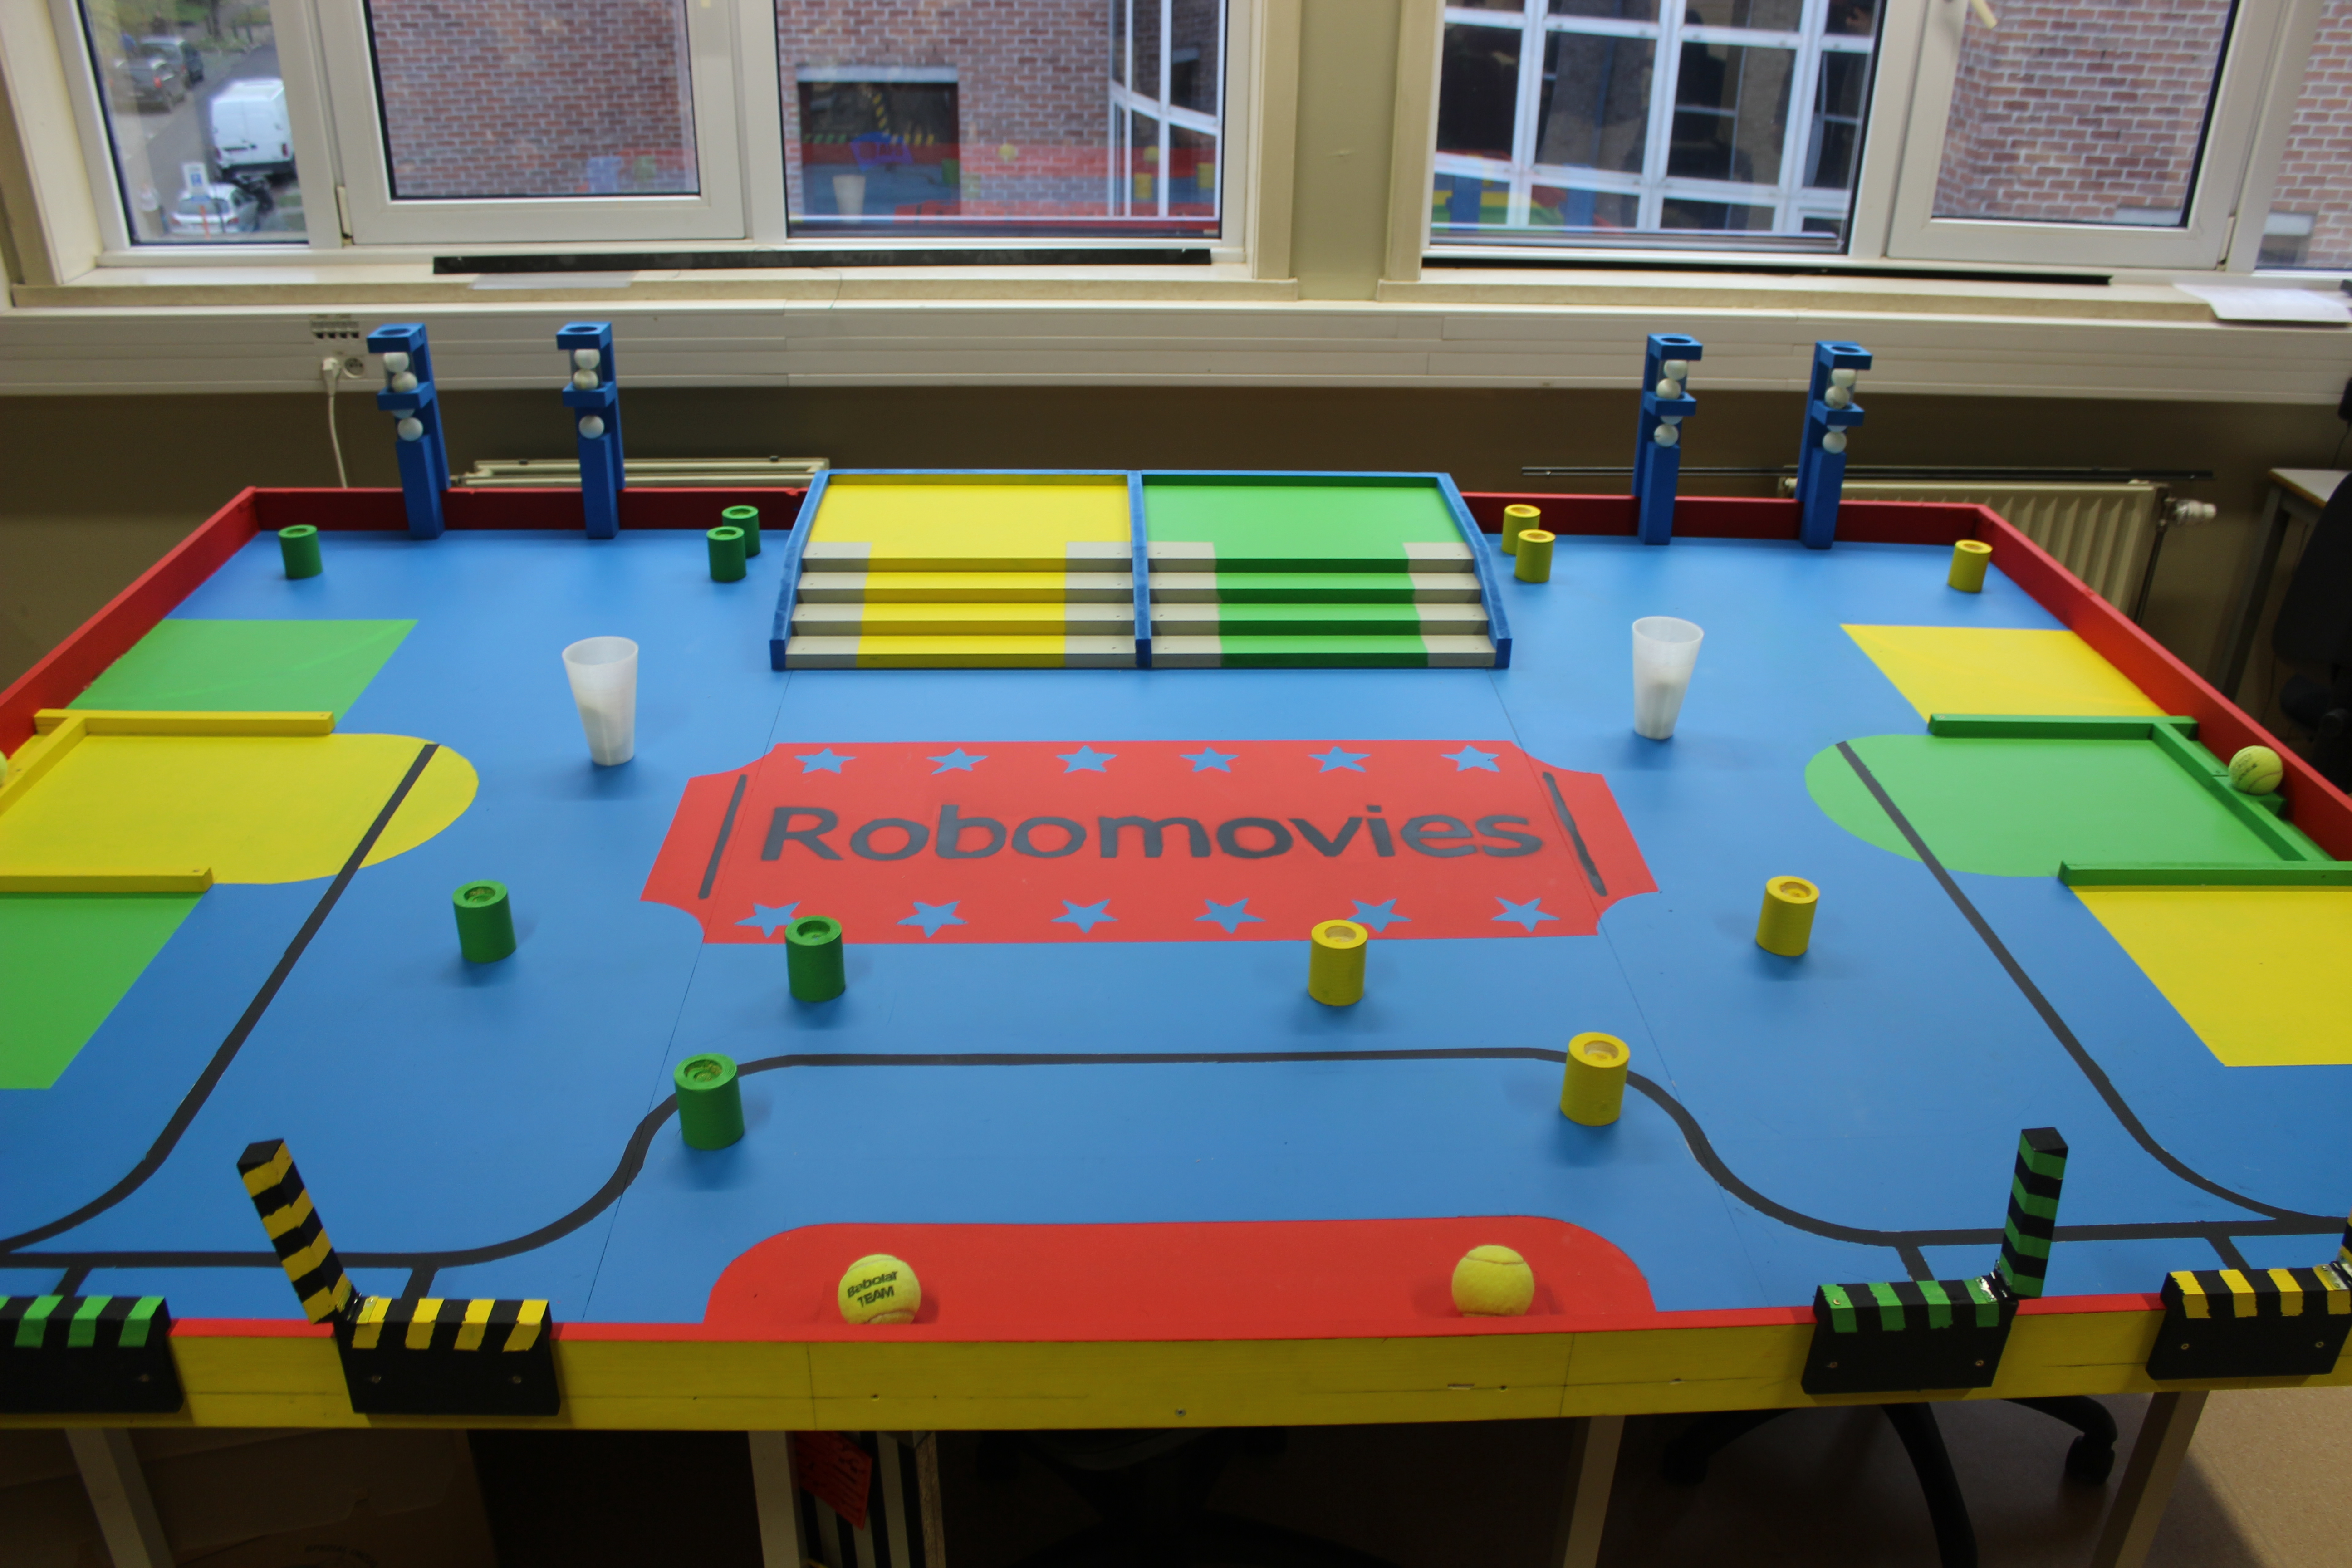
\includegraphics[width=15cm]{Eurobot_Table_1.JPG}
	\caption{Table}
	\label{img:table}
\end{figure}

\subsection{Action des robots}
%~~~~~~~~~~~~~~~~~~~~~~~~~~~~~~~~~~~~~~~~~~~~~~~~~~~~~~~~~~~~
\subsubsection{Introduction}
%~~~~~~~~~~~~~~~~~~~~~~~~~~~~~~~~~~~~~~~~~~~~~~~~~~~~~~~~~~~~
Chaque match est composé de 5 épreuves à réaliser grâce à 1 ou 2 robots indépendants. Aucun contact entre les adversaires n’est autorisé sous peine de malus donc les robots devront être prompts à s’arrêter en cas de rencontre.

\subsubsection{The spotlight}
%~~~~~~~~~~~~~~~~~~~~~~~~~~~~~~~~~~~~~~~~~~~~~~~~~~~~~~~~~~~~
Le robot devra bâtir des spotlights. Pour ce faire, il devra aller récupérer des stands de sa couleur (8 au total) et les amener dans une des zones de construction (1 par équipe + 1 commune).  Ensuite, il suffira d’empiler les stands le plus haut possible et de placer une balle de tennis (4 disponibles, mais communes aux 2 équipes) à son sommet.

\noindent Chaque stand présent dans la zone de construction personnelle rapportera des points mais un seul spotlight peut y être construit. Les autres devront être réalisés dans la zone commune.

\noindent On ne peut en aucun cas interagir avec les stands adverses et un spotlight placé sur la plateforme de la zone commune ne peut être altéré (vol de la balle de tennis) par l’adversaire.

\paragraph{}
Chaque plot rapporte 2 points s’il est correctement placé dans une zone de construction et 3 points bonus par spotlight valide (tour avec balle de tennis).

\subsubsection{The clapperboards}
%~~~~~~~~~~~~~~~~~~~~~~~~~~~~~~~~~~~~~~~~~~~~~~~~~~~~~~~~~~~~
Le robot devra aller fermer les clapperboards correspondant aux couleurs de son équipe qui sont au nombre de 3 (2 proches de sa zone de départ et 1 chez l’adversaire). Il peut se servir de la ligne noire tracée au sol pour se diriger facilement jusqu’aux clapperboards.

\paragraph{}
Cette épreuve rapporte 5 points par clapperboard correctement fermé.

\subsubsection{The popcorn}
%~~~~~~~~~~~~~~~~~~~~~~~~~~~~~~~~~~~~~~~~~~~~~~~~~~~~~~~~~~~~
Le robot devra récolter des popcorns et soit les amener dans sa base et les placer dans la rigole de récupération soit les placer dans un gobelet et l’amener dans une des 3 zones « cinéma » appartenant à son équipe (1 gobelet maximum par zone, le plus rempli sera pris en compte). 

\noindent Les popcorns sont initialement mis dans les gobelets ou dans les machines de distribution. La table proposera 5 verres contenant chacun 4 popcorns et 4 machines avec 5 popcorns.

\noindent Il est nécessaire de savoir que les gobelets placés dans un cinéma peuvent être « volés » par l’équipe adverse.

\paragraph{}
Chaque popcorn présent dans un gobelet placé dans une zone « cinéma » ou placé dans la rigole de la base rapportera 1 point.

\subsubsection{Climbing the red carpet steps}
%~~~~~~~~~~~~~~~~~~~~~~~~~~~~~~~~~~~~~~~~~~~~~~~~~~~~~~~~~~~~
Le robot devra se diriger vers les escaliers situés à l'arrière de la zone de jeu, gravir les marches pour se trouver au sommet à la fin du match.

\paragraph{}
15 points seront attribué en cas de réussite.

\subsubsection{The red carpet}
%~~~~~~~~~~~~~~~~~~~~~~~~~~~~~~~~~~~~~~~~~~~~~~~~~~~~~~~~~~~~
Le robot devra placer de part et d’autre de son escalier un bout de tissu rouge sur les marches de couleurs grises. Pour ce faire, le plus simple sera de monter au sommet et, ensuite, de dérouler le tissu préalablement roulé et mis à bord du robot. 

\paragraph{}
Chaque marche (4 au total x 2) couverte rapportera 2 points et un bonus de 4 points sera offert par volée complètement couverte.

\subsubsection{Bonus/Malus}
%~~~~~~~~~~~~~~~~~~~~~~~~~~~~~~~~~~~~~~~~~~~~~~~~~~~~~~~~~~~~
Toute pénalité impliquera un retrait de 10 points à l'équipe jusqu'à un minimum de 0.
\noindent Il est important se savoir que pour valider un point, le robot ne peut plus avoir d'emprise sur l'objet en question : si en déplacant le robot sur son axe de déplacement principal en impliquant un mouvement de l'objet, celui-ci ne sera pas valide.
\noindent Et, pour finir, 5 points seront attribués à chaque équipe qui n'est pas considérée comme "scratched" : robot présent et fonctionnel.

\subsubsection{Situation Actuelle}
%~~~~~~~~~~~~~~~~~~~~~~~~~~~~~~~~~~~~~~~~~~~~~~~~~~~~~~~~~~~~
Dans notre cas, nous alignerons 2 robots qui s'occuperont chacun de plusieurs tâches distinctes. 

\noindent Le principal s'occupera des 3 premières épreuves : The spotlight, The clapperboards et The popcorn. Tandis que le second s’occupera des escaliers : Climbing the red carpet steps et The red carpet.

\paragraph{}
Pour assurer ces deux dernières opérations, le choix s’est orienté vers l’achat d’un robot à chenille déjà assemblé compatible avec arduino. Nous l’avons choisi notamment pour sa bonne répartition du poids et sa facilité à franchir les marches d’escalier.  

\paragraph{}
Pour le moment, notre attention est dirigée sur The clapperboards et Climbing the red carpet steps qui, en plus de rapporter une bonne quantité de points sans trop de difficulté (3*5 + 15 points), parcoure l'ensemble des fonctionnalités primaires attendues chez nos 2 robots à savoir le déplacement, la détection et la gestion des obstacles, la maitrise de la pince mécanique et l'escalade des marches.

\noindent Pour les autres épreuves, nous n’avons pas encore déterminé l’ordre des actions que le robot effectuera et comment il devra réagir en situation réelle.

\newpage
\section{Architecture}
%Architecture
\subsection{Buts principaux}
%~~~~~~~~~~~~~~~~~~~~~~~~~~~~~~~~~~~~~~~~~~~~~~~~~~~~~~~~~~~~
L'architecture hardware du robot a pour objectif d'être modulable. Cette solution a été retenue afin de pouvoir ajouter des fonctionnalités supplémentaires au cours du projet. L'avantage principal est d'avoir la possibilité de se concentrer sur un module à la fois.

\noindent Quatre modules ont été définis pour permettre au robot de réaliser les actions de bases. Chacun, basé sur une carte électronique propre, sera connecté à la carte principale via un bus de communication (I2C, SPI ou UART). Les modules sont les suivants :

\begin{itemize}
	\item Arduino Master : carte principale qui contrôlera l'ensemble du robot. Elle est à la tête de toutes les autres cartes.;
	\item Arduino Motor : module très important qui commandera les moteurs ;
	\item Raspberry Pi : module qui aura  pour but de voir ce qu'il se passe autour du robot afin de définir les objectifs à atteindre.;
	\item Arduino Bras : carte secondaire qui contrôlera la pince du robot.
\end{itemize}

\paragraph{}
Le fait que l'architecture soit modulable permettra également aux futurs utilisateurs de récupérer un ou plusieurs module pour les exploiter dans leur projet.

\noindent On peut voir les liens entre les différents modules sur la figure~\ref{img:hardware}. On y voit également des éléments tels que la batterie, les moteurs, ou encore les différents capteurs présents sur le robot. Il faut cependant bien avoir en tête que ce schéma n'est qu'une version provisoire qui évoluera avec le projet.

\begin{figure}[!ht]
	\centering
	\includegraphics[width=15cm]{hardware.PNG}
	\caption{Schéma bloc hardware}
	\label{img:hardware}
\end{figure}

\subsection{Choix des cartes}
%~~~~~~~~~~~~~~~~~~~~~~~~~~~~~~~~~~~~~~~~~~~~~~~~~~~~~~~~~~~~
Pour notre robot, nous avons ensemble énuméré les avantages et désavantages de chacune des cartes pour nous faciliter la tâche quand nous devrons les utiliser.

\noindent On peut travailler avec une Rasperry Pi, une Arduino ou encore une DE0 nano, mais quelle est la meilleure ? 

\subsubsection{DE0 nano}
%~~~~~~~~~~~~~~~~~~~~~~~~~~~~~~~~~~~~~~~~~~~~~~~~~~~~~~~~~~~~
\noindent Avantages :
\begin{itemize}
	\item Instantanée;
	\item Carte plus performante que les autres (très puissante);
	\item Nombreuses pins à disposition.
\end{itemize}

\noindent Inconvénients :
\begin{itemize}
	\item Difficulté lors de la programmation (VHDL);
	\item Coût important;
	\item Test Bench à faire manuellement;
	\item Limitée par le nombre de sorties;
	\item Temps de compilation plus lent que les autres cartes.
\end{itemize}

\subsubsection{Raspberry Pi}
%~~~~~~~~~~~~~~~~~~~~~~~~~~~~~~~~~~~~~~~~~~~~~~~~~~~~~~~~~~~~
\noindent Avantages :
\begin{itemize}
	\item Utilisation facile, architecture linux;
	\item Utilisation de la caméra aisée;
	\item OpenCV, très bien documenté.
	\item Elle freeze (Testé en laboratoire).
\end{itemize}

\noindent Inconvénients :
\begin{itemize}
	\item Limitation du nombre pins, besoin d'une carte supplémentaire;
	\item Système exploitation, implique que l'on est pas en temps réel; 
	
\end{itemize}

\subsubsection{Arduino}
%~~~~~~~~~~~~~~~~~~~~~~~~~~~~~~~~~~~~~~~~~~~~~~~~~~~~~~~~~~~~
\noindent Avantages :
\begin{itemize}
	\item Consommation faible : 42mA (0,5W) pour 700mA (3,5W) sur Rpi;
	\item Temps réel (ATmega328 8 bits d'Atmel à 16MHz);
	\item Communautaire et très documentée sur internet;
	\item Programmation aisée en C++;
	\item Communication : module pré-existant.
\end{itemize}

\noindent Inconvénients :
\begin{itemize}
\item 32 Ko d'espace mémoire uniquement (Uno);
\item Impossibilité d'intégrer un module caméra avec une Arduino.
\end{itemize}

\subsection{Nomenclature}
%~~~~~~~~~~~~~~~~~~~~~~~~~~~~~~~~~~~~~~~~~~~~~~~~~~~~~~~~~~~~
Cette liste nous permet d'avoir une vue d'ensemble de ce que nous allons utiliser comme matériel. Cependant, elle n'est pas définitive. En effet, elle sera sujette à quelques modifications (ajout et/ou suppression d'éléments) tout au long du projet. 

\noindent Liste : 
\begin{enumerate}
	\item Roues : 
	\begin{itemize}
		\item 2 roues;
		\item 2 roues codeuses;
		\item Buffer 3,3-5V;
		\item Roue libre.
	\end{itemize}

	\item Moteur : 
	\begin{itemize}
		\item 2 moteurs;
		\item 4 engrenages;
		\item 2 courroies;
		\item Drivers.
	\end{itemize}

	\item  Cartes : 
	\begin{itemize}
		\item Raspberry Pi;
		\item 2 Arduino Uno;
		\item DE0 nano;
		\item Arduino Mega 2560;
		\item Carte ECAM RPI (Buffer);
		\item Carte stratégie, initialisation et démarrage avec corde;
		\item Bouton arrêt urgence.
	\end{itemize}

	\item Alimentation : 
	\begin{itemize}
		\item Carte ECAM.
	\end{itemize}

	\item Capteurs : 
	\begin{itemize}
		\item Line tracking;
		\item 2 Gyroscopes accéléromètre;
		\item 5 Capteurs ultrasonique.
	
	\end{itemize}

	\item Châssis : 
	\begin{itemize}
		\item Vis (quincaillerie);
		\item 3 plaques acier;
		\item Tiges;
		\item Courroie-Poulie;
		\item Plexiglas (carrosserie). 
	\end{itemize}

	\item Système levage pince : 
	\begin{itemize}
		\item Pince modèle ECAM ;
		\item Rail ;
		\item 3 Dynamixel;
		\item 2 poulies crantée avec roulement à billes;
		\item Courroie crantée;
		\item 1 plaque en L pour fixer la Dynamixel du la courroie sur structure.
	\end{itemize}
\end{enumerate}

\newpage
\section{Communications}
\begin{frame}
\frametitle{Communications}
\framesubtitle{Arduino - Arduino}

\begin{description}
\item[I\up{2}C]
\item Transfert à plusieurs esclaves;
\item Fonction;
\item Données.
\end{description}

\begin{table}[!ht]
	\centering
	\begin{tabular}{|c|c|c|c|}
		\hline
		adresse & fonction & data & data \\
		\hline
		7 bits & 4 bits & 4 bits & 8 bits \\
		\hline
	\end{tabular}
	\caption{Trame I\up{2}C}
	\label{tb:TrameI2C}
\end{table}
\end{frame}

\begin{frame}
\frametitle{Communications}
\framesubtitle{Arduino - DE0nano}
\begin{description}
\item[Direct]
\item Appliquer un prescaler;
\item Transfert d'un signal.
\end{description}
\end{frame}

\begin{frame}
\frametitle{Communications}
\framesubtitle{Arduino - Raspberry Pi}
\begin{description}
\item[SPI/UART]
\item Communication entre 2 cartes;
\item Transfert de données.
\end{description}
\end{frame}


\newpage
\section{Régulation}
\begin{frame}
\frametitle{Régulation}
\framesubtitle{Introduction}
Quelques questions à se poser :
\begin{itemize}
	\item Où veut-on aller ?
	\item Comment commander les moteurs ?
	\item Vers où le robot se dirige-t-il ? Où est-il par rapport à l'objectif ?
	\item Il y a-t-il un obstacle devant le robot ?
	\item Pourquoi a-t-on besoin d'une régulation ?
\end{itemize}
\end{frame}

\begin{frame}
\frametitle{Régulation}
\framesubtitle{Consigne et commande des moteurs}
La consigne est reçue via l'I\up{2}C, on a disposition :
\begin{itemize}
	\item La fonction (4bits), choix de la commande;
	\item Les données (12bits), distance à parcourir.
\end{itemize}
\begin{table}[!ht]
	\centering
	\begin{tabular}{|l|cc|cc|}
		\hline
		& DIR1 & DIR2 & PWM1 & PWM2 \\
		\hline
		Forward & 1 & 1 & \multicolumn {2}{c|}{Variable} \\
		\hline
		Backward & 0 & 0 & \multicolumn {2}{c|}{Variable} \\
		\hline
		Turn Left & 1 & 0 & \multicolumn {2}{c|}{Variable} \\
		\hline
		Turn Right & 0 & 1 & \multicolumn {2}{c|}{Variable} \\
		\hline
		Stop & \multicolumn {2}{c|}{X} & 0 & 0 \\
		\hline
	\end{tabular}
	\caption{Commandes des moteurs}
\end{table}
\end{frame}

\begin{frame}
\frametitle{Régulation}
\framesubtitle{Roues codeuses et capteurs ultrasons}
Capteurs ultrasons : uniquement en cas d'arrêt d'urgence.\\
Roues codeuses :
\begin{itemize}
	\item 1024 tics par tour ;
	\item 20 cm par tour.
\end{itemize}
\begin{figure}[!ht]
	\centering
	\includegraphics[scale=0.5]{roues_codeuses.png}
	\caption{Signal des roues codeuses}
\end{figure}
\end{frame}

\begin{frame}
\frametitle{Régulation}
\framesubtitle{Schéma bloc}
\begin{figure}[!ht]
	\centering
	\includegraphics[scale=0.28]{simulink.jpg}
	\caption{Schéma bloc de la régulation des moteurs}
	\label{img:simulink}
\end{figure}
\end{frame}

\begin{frame}
\frametitle{Régulation}
\framesubtitle{Coefficients Kp et Kig}
\begin{description}
	\item[Kp] Coefficient proportionnel du déplacement; 
			\hfill \\ Ralentir la commande en se rapprochant. 
	\item[Kig] Coefficient intégrateur du glissement;
			\hfill \\ Éviter les variations entre la rotation des moteurs et la rotation des roues.
\end{description}
\end{frame}

\newpage
\section{Châssis}
%Chassis
\subsection{Introduction}
%~~~~~~~~~~~~~~~~~~~~~~~~~~~~~~~~~~~~~~~~~~~~~~~~~~~~~~~~~~~~
L'opération châssis n'a débuté qu'après avoir défini avec toute l'équipe quelles actions le robot devra accomplir. La décision s'est prise principalement en fonction du nombre de points que cela pourrait nous rapporter en tenant compte de la complexité demandée et du temps que celle-ci demande. 

\paragraph{}
Ensemble, nous avons donc conclu qu'une pince était amplement suffisante pour réaliser 3 des 5 actions demandés pour le concours. Cette année nous avons décidé d'utiliser deux robots pour répondre à nos besoins : un robot avec un mécanisme élévateur composé de la pince et un robot chenille. Les actions définies, nous avons pu mettre en place les techniques choisies pour les accomplir.

\subsection{Objectifs}
%~~~~~~~~~~~~~~~~~~~~~~~~~~~~~~~~~~~~~~~~~~~~~~~~~~~~~~~~~~~~
Conception d'une base adéquate capable de recevoir une pince mécanique et les nouveaux moteurs acquis cette année. 

\paragraph{}
La pince mécanique doit être capable de soulever un objet, de le transporter à un endroit souhaité et d'empiler des objets les uns sur les autres.

\subsection{Étude de l'existant}
%~~~~~~~~~~~~~~~~~~~~~~~~~~~~~~~~~~~~~~~~~~~~~~~~~~~~~~~~~~~~
Après une étude et un choix de ce qui est à notre disposition. Nous avons décidé de nous baser sur le principe du mécanisme d'élévation présent sur un châssis déjà monté afin d'assurer le déplacement vertical de la pince. Malheureusement, ce châssis ne peut être réutilisé vu qu'il n'appartient pas à l'ECAM.

\paragraph{}
L'autre châssis, celui de l'ECAM n'est plus adéquat avec ce que l'on a besoin étant donné que les nouveaux moteurs ont été dimensionnés avec le réducteur adéquat ce qui allonge l'emplacement du support moteur.

\subsection{Mécanisme d'élévation}
%~~~~~~~~~~~~~~~~~~~~~~~~~~~~~~~~~~~~~~~~~~~~~~~~~~~~~~~~~~~~
L'élévation sera donc assurée par un rail constitué d'un guidage et d'une poulie à chacune de ces extrémités dont la liaison est assurée par une courroie crantée contrôlée par un servomoteur. Une pièce métallique est attachée à la courroie et assure le déplacement de la pince.  

\noindent On peut voir à la figure~\ref{fig:Chariot} un élément représentatif qui a été réalisé sous CATIA.

\begin{figure}[!ht]
	\centering
		\includegraphics{chariot.png}
	\caption{Mécanisme d'élévation}
	\label{fig:Chariot}
\end{figure}

\noindent Ce mécanise correspondait bien avec ce dont on a besoin comme par exemple :  

\begin{itemize}
	\item Montée à la hauteur de 200mm pour atteindre le distributeur de pop-corn;
	\item Ou encore monter à plus de 210mm afin d'empiler par exemple 3 pieds et placer une balle de tennis pour réaliser le spot de lumière.
\end{itemize}

\paragraph{}
Ainsi nous sommes partis sur ce principe et avons réalisé une base prévue pour recevoir le mécanisme d'élévation, notamment la pince dont les servomoteurs seront implémentés de manière à se retrouver à l'intérieur de la surface totale du châssis. Ceci est nécessaire afin de minimiser la longueur totale du robot et d'éviter que la pince ressorte trop vers l'extérieur à cause de la présence des servomoteurs.

\subsection{Support moteur}
%~~~~~~~~~~~~~~~~~~~~~~~~~~~~~~~~~~~~~~~~~~~~~~~~~~~~~~~~~~~~
Pour la mise en place du moteur, nous avons totalement changé le système d'accouplement de la roue au moteur par rapport aux années précédentes. Nous avons choisi l'option la plus simple c'est-à-dire lier le moteur a la roue directement sans passer par la courroie et la poulie de réduction, étant donné qu'un réducteur existe déjà dans le moteur.

\paragraph{}
La seule pièce qu'on a dû créer est le support du moteur (figure~\ref{fig:support}) vu que la fixation du moteur sur le support exige une grande précision en tenant compte des tolérances, nous nous sommes basés  sur une pièce déjà existante. En la modifiant, nous avons créé un système simple pour la mise en place des moteurs et en même temps solide, surtout que le moteur présente un couple élevé après l'étage de réduction de la vitesse.

\begin{figure}[!ht]
	\centering
		\includegraphics{support.jpg}
	\caption{Support Moteur}
	\label{fig:support}
\end{figure}

\subsection{Assemblage des différents éléments}
%~~~~~~~~~~~~~~~~~~~~~~~~~~~~~~~~~~~~~~~~~~~~~~~~~~~~~~~~~~~~
Afin de mieux visualiser la longueur totale de notre robot et de minimiser l'emplacement, un modèle de notre robot a été réalisée sous CATIA.

\vspace{5mm}
\begin{figure}[!ht]
	\centering
		\includegraphics{assemblage.png}
	\caption{Éléments assemblés}
	\label{fig:assemblage}
\end{figure}

\paragraph{}
Le châssis du robot qui sera construit en P2 sera constitué de 2 plaques :
\begin{itemize}
	\item La base qui sera réalisée en aluminium sera composée des éléments comme le moteur, la batterie et le driver; 
	\item La deuxième plaque sera réalisée soit en PVC soit en aluminium, celle-ci sera constituée de toutes les cartes comme l'alimentation (partie d'en dessous) la Raspberry Pi, Arduino Mega, Arduino Uno et DE0-nano.
\end{itemize}

\paragraph{}
La réalisation de la pince a été entreprise par Nehri Nabil en même temps que la réalisation de la base. La création des supports pour les cartes électroniques n'a pas encore été réalisée notamment dû à l'incertitude de l'emplacement définitif des cartes. 

\paragraph{}
À ce stade, nous ne savons pas si de nouvelles cartes électroniques peuvent encore être créées ou modifiées. Le positionnement sera ajusté par étape d'implémentation en P2.

\noindent Le robot présente approximativement comme valeurs maxima une longueur de 240mm sans la pince et 370mm si on tient compte de celle-ci. Il fait également 340mm de largeur contre un peu plus de 300mm de hauteur.

\subsubsection{Inconvénients}
\begin{itemize}
	\item On ne peut faire qu'une action à la fois car 3 actions dépendent de la pince;
	\item Peut présenter un souci pour se positionner face à un objet à cause des capteurs qui doivent être présents pour assurer son positionnement;
	\item  La pince demande deux servomoteurs qui rendent les commandes plus difficiles mais offrent un meilleur résultat;
	\item L'encombrement de la pince est de 170mm de longueur ce qui est un handicap, elle augmente considérablement la taille du robot.
\end{itemize}

\subsection{Problèmes rencontrés}
%~~~~~~~~~~~~~~~~~~~~~~~~~~~~~~~~~~~~~~~~~~~~~~~~~~~~~~~~~~~~
Le principal souci rencontré a été que si l'on utilise une version supérieure de CATIA, il devient impossible d'ouvrir un fichier d'une version antérieure. Malheureusement, nous nous sommes rendus compte de ceci une fois la mise en commun des différentes réalisations.

\subsection{Annexes}
%~~~~~~~~~~~~~~~~~~~~~~~~~~~~~~~~~~~~~~~~~~~~~~~~~~~~~~~~~~~~
Tout les plans, ainsi que toutes les réalisations avec CATIA se trouvent dans le dossier Éléments CATIA déposé sur silicium.

\newpage
\section{Pince}
\begin{frame}
\frametitle{Pince}
\framesubtitle{Dynamixels 1/2}
\begin{description}
	\item [Caractéristiques]
	\item Moteur électrique de petite taille;
	\item Réducteur pour diminuer la vitesse et augmenter le couple;
	\item  Commande : Largeur impulsion (PWM);
	\item  Temps impulsion : détermine angle à fournir;
	\item  Angle d'ouverture : 0-300°.
\end{description}
\end{frame}

\begin{frame}
\frametitle{Pince}
\framesubtitle{Dynamixels 2/2}
\begin{figure}[!ht]
	\includegraphics[scale=0.5]{instu.png} 
	\caption{Instruction Packet}
\end{figure}
\end{frame}

\begin{frame}
\frametitle{Pince}
\framesubtitle{Objectifs}
\begin{description}
	\item [Problématique]
	\item Déterminer les tâches;
	\item Pouvoir la contrôler facilement (Software);
	\item Budget.
	\item [Choix]
	\item Design ECAM.
\end{description}
\end{frame}

\begin{frame}
\frametitle{Pince}
\framesubtitle{Contrôle}
\begin{description}
	\item [Comment contrôler les Dynamixels ?]
	\item Libraire Savage;
	\item Arduino.
	\item [Fonctions]
	\item Dynamixel.movespeed(ID,Position,Speed)
	\item Dynamixel.move(ID,Position)
\end{description}
\end{frame}

\begin{frame}
\frametitle{Pince}
\framesubtitle{Catia}
\begin{description}
	\item [En pratique]
	\item Premier test : deux doigts;
	\item Idée : pinces à cheveux;
	\item Deuxième test : 3-2 doigts avec croisement.
\end{description}
\end{frame}


\newpage
\section{Dimensionnement des moteurs}
\begin{frame}
\frametitle{Moteur}
\framesubtitle{Dimensionnement}
\begin{description}
\item[Régime permanent]
\item En régime permanent l'accélération est nulle;
\item $Fm - Fr = m \times \overrightarrow{a} = 0$.
\item[Résultats]
\item $P = Cm \times \omega m = 694\frac {rad}{s}  \times 0.02943N = 20.42W$;
\item Vitesse maximale du robot $V = 5\frac{km}{h} = 1.38\frac{m}{s}$.
\end{description}
\end{frame}

\begin{frame}
\frametitle{Moteur}
\framesubtitle{Dimensionnement en tenant compte de l'accélération}
\begin{itemize}
\item Pour simplifier les calculs on suppose qu'on atteint la vitesse du régime, c'est-à-dire 1.38m/s en 1s;
\item $Fm - Fr = m \times \overrightarrow{a} = 10kg \times 1.38\frac{m}{s^{2}} = 13.8N$;
\item $Fm = Fr + 13.8N = 13.8 + 17.715 = 28.5N$ ;
\item $Croue = Fr \times r = 28.5N  \times 0.04m = 1.14Nm$, $r = 0.04m$ rayon de la roue ;
\item $Cmoteur = \frac {Croue}{20} = 57mNm$;
\item $P = Cm \times Wm = 0.057mNm \times 694\frac{rad}{s} = 39.7W$;
\item $2 moteurs \rightarrow 20 Watts par moteur$.
\end{itemize}
\end{frame}

\begin{frame}
\frametitle{Moteur}
\begin{figure}[!ht]
	\centering
	\includegraphics[scale=0.7]{Moteur.PNG}
	\caption{Moteur}
\end{figure}
\end{frame}

\begin{frame}
\frametitle{Moteur}
\begin{figure}[!ht]
	\centering
	\includegraphics[scale=0.6]{Gearhead.PNG}
	\caption{Gearhead}
\end{figure}
\end{frame}

\begin{frame}
\frametitle{Moteur}
\begin{figure}[!ht]
	\centering
	\includegraphics[scale=0.6]{Encoder.PNG}
	\caption{Encoder}
\end{figure}
\end{frame}

\begin{frame}
\frametitle{Driver}
\end{frame}

\newpage
\chapter{Perspectives}
\begin{frame}
\frametitle{Perspectives}
\begin{description}
\item[OpenCV] Traitement d'image;
\item[Line Tracking] Suiveur d'une ligne;
\item[Pince] Prendre/Bouger/Monter des objets;
\item[Position] Système de position sur la table.
\end{description}
\end{frame}


\end{document}